\clearemptydoublepage
\chapter{Présentation du sujet} 
\minitoc
\emph{Nous avons choisi d'aborder ce sujet d'une manière différente de l'approche classique. Dans un premier temps, nous n'avons pas cherché à répondre à un besoin fonctionnel mais à une interrogation d'ordre philosophique : 
\begin{center}
\og Est-il possible de synthétiser dans une machine des processus cognitifs se rapprochant de ceux de l'être humain ? Si oui, comment ? \fg{}
\end{center}
C'est une démarche réellement différente de celle proposée par l'intelligence artificielle dite \og moderne \fg{}\footnote{Cf. Russell S. et Norvig P. (2009 -- 3rd Ed.), \og Artificial intelligence : a modern approach \fg{}, Prentice Hall, 0-13-604259-7}, la tendance de nos jours étant de suivre une voie plus pragmatique visant à aboutir à des systèmes dits \og rationnels \fg{}, c'est à dire se comportant de manière optimale vis-à-vis d'une mesure de performance donnée. Ce nouveau paradigme s'est constitué en réaction à une IA juvénile atteinte par l'ampleur de ces ambitions. À l'origine, les équipes de recherche pensaient pouvoir construire rapidement des systèmes égalant les capacités humaines, mais les résultats ne sont pas arrivés à la hauteur de leurs espérances. Leurs investisseurs déçus ont alors provoqué durant les années 1970-1990 les \og hivers de l'IA \fg{} en retirant la majorité de leurs soutiens financiers.}

\emph{Sans oublier cette leçon d'humilité, nous avons fait le choix d'essayer de renouer avec une approche biomimétique.}

\section{Objectifs} 
Notre objectif lors de ce TER sera donc de construire une intelligence artificielle basé sur une approche biomimétique, c'est à dire que nous tenterons d'approcher un problème d'intelligence artificielle à partir de mécanismes connues du fonctionnement du cerveau. Dans un premier temps, nous devrons étudier et assimiler le modèle de la conscience présenté dans le rapport sur lequel se base notre TER. Dans un deuxième temps, il nous faudra décidé d'un domaine sur lequel appliqué notre IA. Ensuite, nous formaliserons le modèle général pour l'appliquer au domaine choisi. Enfin, nous implémenterons notre finalisation. Et Finalement, nous devrons prendre du recule par rapport à notre travail afin d'effectuer un travail d'évaluation de façon objective.

\section{Pourquoi une approche cognitive?} 
L’Homme a toujours cherché à comprendre et à reproduire les mécanismes naturels qui l'entourent. Un des domaines les plus passionnants reste celui de l'étude du cerveau. Qu'il soit humain ou animal, nous restons fascinés par sa capacité à analyser, à comprendre et à généraliser les problèmes que posent ou \og proposent \fg{} l'environnement.

Afin de se rapprocher du fonctionnement du cerveau, nous traiterons le sujet de notre TER avec les approches suivantes.


\subsection{Une approche par apprentissage}

Une des principales caractéristiques de l'intelligence, et sûrement une des plus importantes, est la capacité d'apprentissage. C'est pourquoi notre IA devra améliorer ses performances avec le temps en se basant sur ses expériences. Nous pouvons citer Alain Bonnet qui dans son livre «~L'intelligence artificielle, promesses et réalités~», paru en 1984, écrit : «~Les programmes devront apprendre  avec l'expérience et s'auto-améliorer sur de simples jugements de leurs performances que les experts humains fourniront. Dans un premier temps, ils pourront améliorer leurs connaissances et dans un deuxième, leurs mécanismes d'utilisation de ces connaissances, c'est à dire leurs stratégies de plus haut niveau.~».


\subsection{Une approche par reconnaissance de formes}

La reconnaissance de formes dans notre environnement est une autre des principales capacités de notre cerveau. En effet, le cerveau interprète les informations visuels qui lui sont transmises et en extrait des concepts ou formes connues. Par exemple, pour un être humain, les formes tels que \og chaise \fg{}, \og porte \fg{}, \og fenêtre \fg{}, etc, sont automatiquement reconnues par notre cerveau.



\section{Un modèle de représentation de la conscience}
\label{un_modele_de_representation_de_la_conscience}
Dans le but de concrétiser cette approche, nous nous sommes inspirés du travail réalisé par \mbox{Guillaume} \mbox{Tisserant}, \mbox{Guillaume} \mbox{Maurin}, \mbox{Ndongo} \mbox{Wade} et \mbox{Anthony} \mbox{Willemot}. La figure~\ref{modele_original} présente la structure de la conscience artificielle décrite dans cette étude. Celle-ci conserve la plupart des caractéristiques d’une conscience humaine grâce à des recherches sur de nombreux travaux comme ceux de Freud et de Laborit\footnote{Henri Laborit (1914--1995): Médecin chirurgien et neurobiologiste.}.

\begin{figure}[H] 
\centering
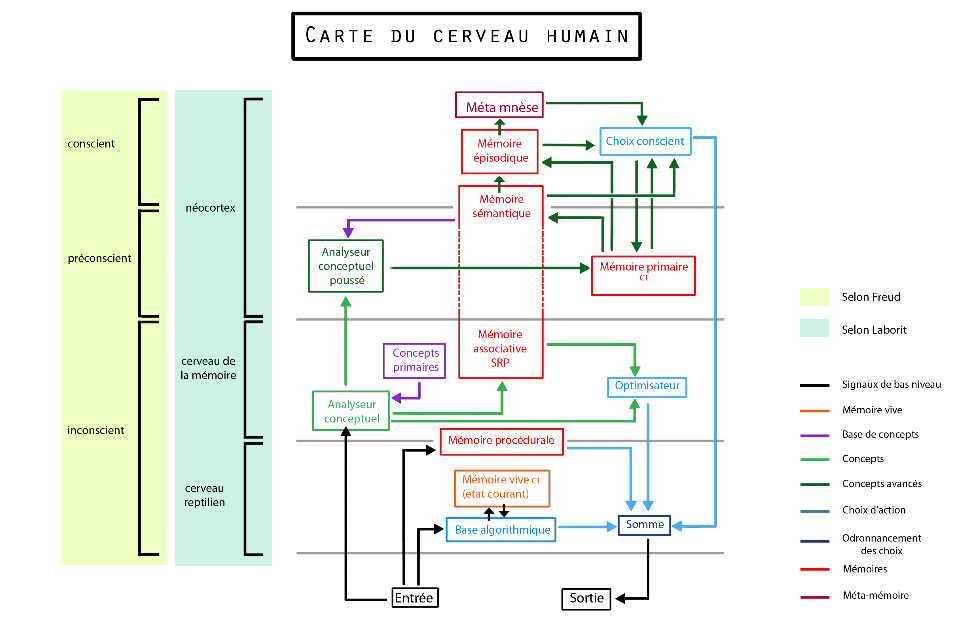
\includegraphics[width=\textwidth]{files/modele_original} 
\caption{Schéma du modèle de représentation de la conscience.} 
\label{modele_original}
\end{figure}

Cette représentation peut être vue comme un empilement de couches : l'inconscient se situant au plus bas et le conscient au plus haut.

\subsection{L'inconscient}
L'inconscient est composé de deux niveaux : le cerveau reptilien et le cerveau de la mémoire.

\subsubsection{Le cerveau reptilien}

C'est la couche la plus basse du modèle.

\paragraph{Les entrées/sorties}
Les entrées permettent au cerveau d'acquérir deux types d'informations :
\begin{itemize}
\item les percepts externes, émis par l'environnement et perçus par les cinq sens,
\item les percepts internes, comme les pulsions, etc. 
\end{itemize}

Les sorties assurent la transmission des informations produites par le cerveau au reste du corps.

\paragraph{La base algorithmique} Il s'agit d'une base simple assurant une réaction rapide à des entrées simples, en produisant des sorties simples. C'est cette partie qui stocke les réflexes innés présents chez les êtres vivants. 

\paragraph{La mémoire procédurale} Elle permet de construire des automatismes en fonction du vécu. Par exemple, selon un schéma essai échec, un bébé apprendra à marcher en utilisant sa mémoire procédurale.

\subsubsection{Le cerveau de la mémoire} Cette couche est plus
complexe que la dernière. Elle est composée d'un analyseur conceptuel, d'une mémoire
associative et d'un optimisateur.

\paragraph {L'analyseur conceptuel} Il analyse des entrées en dur à une base de
données de concepts primaires (comme la faim, la soif, le plaisir, la fatigue, la joie, une odeur
nauséabonde, un bruit violent, etc.).
\paragraph {La mémoire associative} Elle assure l'association de concepts primaires
entre eux. Elle permet par exemple à un animal vivant dans un milieu contenant des prédateurs
bruyants d’associer le concept de danger au bruit émit par le prédateur.
\paragraph {L’optimisateur} Il a pour vocation d’optimiser un concept qui peut
se traduire par le bien-être. Prenons l’exemple précédent : si l'animal sait que l’approche d’un prédateur réduit le bien-être, et que le fait de courir peut éloigner le
prédateur et donc faire remonter le bien-être, alors l'optimisateur permettra à l'animal d'inférer l’action de fuir.

\subsection{Le Néocortex : la préconscience et la conscience}
Les couches faisant partie du néocortex représentent la préconscience et la
conscience. C'est en montant dans ces éléments que l'on s'approche de la cognition humaine.

\subsubsection{Le préconscient} Cette couche est constitué d'un analyseur
conceptuel sémantique et des mémoires primaire et sémantique.

\paragraph{L'analyseur conceptuel sémantique} Il manipule des concepts d'un niveau
supérieur à ceux manipulés par l’analyseur conceptuel du cerveau de la mémoire. Il permet la
traduction de concepts primaires en concepts complexes, qui seront stockés en mémoire
sémantique.

\paragraph{La mémoire sémantique} Elle contient une base de concepts avancés, construite sous forme de treillis, permettant l'association de concepts.

\paragraph{La mémoire primaire} Cette mémoire contient un nombre de concepts
sémantiques limité. Elle joue le rôle d'une mémoire à court terme qui stocke tout ce dont la conscience est en train de manipuler. La mémoire primaire peut recevoir des informations de l’analyseur conceptuel poussé, qui lui envoie les concepts se trouvant dans l’environnement, ou directement par la réflexion consciente, qui choisit d’y stocker un concept sur lequel une réflexion est nécessaire.

\paragraph{La gestion de la mémoire sémantique} Les concepts en mémoire primaire sont instantanément copiés en mémoire sémantique. Toutes les informations qui passent en
mémoire primaire y sont transmit. Cependant, les informations accumulées peuvent être oubliées.
L'oublie d'un concept dépend de l'activité de ce dernier en mémoire primaire.

\subsubsection{Le conscient}
Cette partie regroupe les modules les plus avancés du modèle : la mémoire épisodique, la métamnèse et le choix conscient.

\paragraph{La mémoire épisodique} Il s'agit d'une mémoire des situations, qui permet la remémoration évènements et des émotions vécues sous formes de concepts sémantiques. Les concepts stockés proviennent à la fois des percepts et de l’état interne de la personne au moment de l'événement. Elle gère la persistance au même titre que la mémoire sémantique.

\paragraph{La métamnèse} C'est la mémoire de la mémoire. Son rôle est de stocker la
façon dont les éléments se sont enchaînés dans la mémoire épisodique.

\paragraph{Le choix conscient} (ou réflexion consciente) Il peut être vu comme un optimisateur de haut niveau, maniant des concepts poussés, et de natures différentes. Grâce à la métamnèse, il peut utiliser des séries de situations, et même imaginer des situations passées, présentes ou futures pour prendre des décisions. Il est ainsi capable de comparer des situations imaginaires et choisir celle vers laquelle il a envie de tendre. Il a aussi la capacité à réfléchir sur des concepts abstraits, comme sur ses réflexions passées. Il est capable d'analyser son propre fonctionnement du moment où il arrive à le retranscrire sous forme de concepts.

\subsection{Synthèse}
L’objet représenté par \textbf{Somme} dans la couche du cerveau reptilien est une simplification du schéma retour. Il représente la transformation de tous les signaux en signaux de bas niveaux, et gère leur somme pour choisir lesquels inhiber et lesquels transmettre en sortie. Son fonctionnement nécessite d'arriver à combiner les signaux entre eux. Par exemple, si une personne choisit de fumer dans le choix conscient, il doit récupérer la façon d'allumer un briquet dans la mémoire procédurale.
